\chapter{Letterrekenen en vergelijkingen}\label{ch:g8:equations}

In het derde leerjaar van deze reeks kwamen letters aan bod en leerde je
eenvoudige uitdrukkingen herleiden (\cref{ch:g7:literal}). Dit hoofdstuk voegt
de twee vaardigheden toe die algebra krachtig maken: \emph{haakjes wegwerken}
in \omterm{def:g2:mult:def}{producten}, en het \emph{oplossen van \omterm{def:g8:equations:def}{vergelijkingen}} --- het getal vinden dat
achter de letter schuilgaat.

\section{Haakjes wegwerken}

\begin{theorem}[Enkele en dubbele distributiviteit]\label{thm:g8:equations:expand}
Voor alle getallen geldt:
\[
k(a + b) = ka + kb,
\qquad
(a + b)(c + d) = ac + ad + bc + bd .
\]
\end{theorem}

\begin{proof}
De eerste regel is \cref{thm:g7:priorities:distributivity}, tekens inbegrepen:
$k$ en de termen mogen negatief zijn (\cref{ch:g8:negprod}). Voor de tweede pas
je de eerste regel twee keer toe, met $(c + d)$ als één getal:
\[
(a + b)(c + d) = a(c + d) + b(c + d) = ac + ad + bc + bd .
\qedhere
\]
\end{proof}

\begin{example}\label{ex:g8:equations:expand}
Let bij elke term op het teken:
\begin{align*}
3(2x - 5) &= 6x - 15, \\
-2(4x - 7) &= -8x + 14
&& \text{(een minteken vooraan keert beide tekens om)}, \\
(x + 3)(x + 5) &= x^2 + 5x + 3x + 15 = x^2 + 8x + 15, \\
(2x - 1)(x - 4) &= 2x^2 - 8x - x + 4 = 2x^2 - 9x + 4 .
\end{align*}
\end{example}

\begin{omfigure}
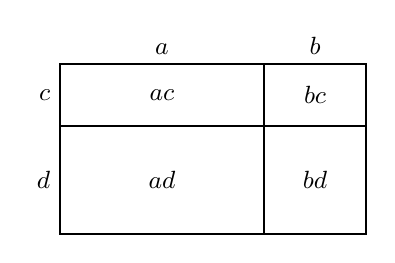
\begin{tikzpicture}[scale=0.72]
  \draw[thick] (0,0) rectangle (5.4,3.0);
  \draw[thick] (3.6,0) -- (3.6,3.0);
  \draw[thick] (0,1.9) -- (5.4,1.9);
  \node[font=\small] at (1.8,2.45) {$ac$};
  \node[font=\small] at (4.5,2.45) {$bc$};
  \node[font=\small] at (1.8,0.95) {$ad$};
  \node[font=\small] at (4.5,0.95) {$bd$};
  \node[above, font=\small] at (1.8,3.0) {$a$};
  \node[above, font=\small] at (4.5,3.0) {$b$};
  \node[left, font=\small] at (0,2.45) {$c$};
  \node[left, font=\small] at (0,0.95) {$d$};
\end{tikzpicture}

{\small Dubbele distributiviteit als \omterm{def:g6:measure:area}{oppervlakte}: de rechthoek
$(a+b) \times (c+d)$ valt uiteen in vier kleinere rechthoeken --- één per term
van het \omterm{def:g2:mult:def}{product}.}
\end{omfigure}

\begin{method}[Haakjes wegwerken en herleiden]\label{met:g8:equations:reduce}
\begin{enumerate}
  \item Werk elk \omterm{def:g2:mult:def}{product} uit en schrijf elke term met zijn teken;
  \item neem gelijksoortige termen samen ($x^2$ bij $x^2$, $x$ bij $x$, getallen
        bij getallen);
  \item controleer met een waarde: vul bijvoorbeeld $x = 2$ in, in de
        oorspronkelijke uitdrukking en in het resultaat --- gelijke uitkomsten
        halen de meeste fouten eruit.
\end{enumerate}
\end{method}

\section{Vergelijkingen oplossen}

\begin{definition}[Vergelijking]\label{def:g8:equations:def}
Een \emph{vergelijking}\index{vergelijking} is een gelijkheid met een onbekend
getal, dat je $x$ noemt (of een andere letter). Haar \emph{oplossen} betekent:
alle waarden van $x$ vinden waarvoor de gelijkheid waar is --- de
\emph{oplossingen}.
\end{definition}

\begin{theorem}[Balansregels]\label{thm:g8:equations:balance}
Een \omterm{def:g8:equations:def}{vergelijking} houdt precies dezelfde oplossingen wanneer:
\begin{enumerate}
  \item bij beide leden hetzelfde getal wordt opgeteld (of ervan afgetrokken);
  \item beide leden met hetzelfde getal, \emph{verschillend van \omterm{def:g1:counting:zero}{nul}}, worden
        vermenigvuldigd (of erdoor gedeeld).
\end{enumerate}
\end{theorem}
\admitted

\begin{omfigure}
\begin{tikzpicture}[scale=0.9]
  \draw[thick] (0,0) -- (0,0.5);
  \draw[thick] (-2.6,0.5) -- (2.6,0.5);
  \draw[thick] (-0.5,0) -- (0.5,0);
  \draw[thick] (-2.2,0.5) -- (-2.2,0.75);
  \draw[thick] (2.2,0.5) -- (2.2,0.75);
  \draw[omDef, fill=omDef!15] (-2.8,0.75) rectangle (-1.6,1.45);
  \node[font=\small] at (-2.2,1.1) {$x{+}3$};
  \draw[omThm, fill=omThm!15] (1.75,0.75) rectangle (2.65,1.45);
  \node[font=\small] at (2.2,1.1) {$8$};
  \node[below, font=\small] at (0,-0.25)
    {haal $3$ uit beide schalen: $x = 5$};
\end{tikzpicture}

{\small Een \omterm{def:g8:equations:def}{vergelijking} is een balans in evenwicht: wat je met de ene schaal
doet, moet je ook met de andere doen, en dan blijft het evenwicht --- de
gelijkheid --- bestaan.}
\end{omfigure}

\begin{method}[Een eerstegraadsvergelijking oplossen]\label{met:g8:equations:solve}
\begin{enumerate}
  \item Werk indien nodig de haakjes weg en herleid elk lid;
  \item tel bij beide leden op of trek van beide leden af, tot de
        $x$-termen in het ene lid staan en de losse getallen in het andere;
  \item herleid, en deel dan beide leden door de coëfficiënt van $x$;
  \item \emph{controleer} door de gevonden waarde in de oorspronkelijke
        \omterm{def:g8:equations:def}{vergelijking} in te vullen.
\end{enumerate}
\end{method}

\begin{example}\label{ex:g8:equations:solve}
Los $7x - 5 = 4x + 16$ op:
\begin{align*}
7x - 5 &= 4x + 16 \\
7x - 4x &= 16 + 5
&& \text{(bij beide leden $5$ optellen en $4x$ aftrekken)} \\
3x &= 21 \\
x &= 7 && \text{(beide leden door 3 delen).}
\end{align*}
Controle: linkerlid $7 \times 7 - 5 = 44$; rechterlid
$4 \times 7 + 16 = 44$. De oplossing is $7$.
\end{example}

\begin{example}[Met haakjes en negatieve getallen]\label{ex:g8:equations:brackets}
Los $3(x - 4) = 5 - 2(x + 1)$ op:
\begin{align*}
3x - 12 &= 5 - 2x - 2 && \text{(haakjes in beide leden wegwerken)} \\
3x - 12 &= 3 - 2x && \text{(herleiden)} \\
5x &= 15 && \text{($2x + 12$ bij beide leden optellen)} \\
x &= 3 .
\end{align*}
Controle: $3(3 - 4) = -3$ en $5 - 2(3+1) = 5 - 8 = -3$. \quad Oplossing:
$3$.
\end{example}

\begin{method}[Een vraagstuk met een vergelijking oplossen]\label{met:g8:equations:problem}
\begin{enumerate}
  \item Kies de onbekende: ``zij $x$ het aantal \dots'' (de gevraagde grootheid,
        of een eenvoudiger grootheid die ermee samenhangt);
  \item zet het verhaal om in een \omterm{def:g8:equations:def}{vergelijking};
  \item los die op;
  \item interpreteer: antwoord in een volle zin op de gestelde vraag, met
        eenheden, en toets het antwoord aan het verhaal.
\end{enumerate}
\end{method}

\begin{example}\label{ex:g8:equations:problem}
Lucas is $4$ jaar ouder dan zijn zus; samen zijn ze $26$ jaar. Zij $x$ de
leeftijd van de zus; dan is Lucas $x + 4$ jaar, en
\[
x + (x + 4) = 26
\ \Longrightarrow\
2x + 4 = 26
\ \Longrightarrow\
2x = 22
\ \Longrightarrow\
x = 11 .
\]
De zus is $11$, Lucas is $15$. Controle: $11 + 15 = 26$ en
$15 - 11 = 4$.
\end{example}

\section{Ordening en ongelijkheden}

\begin{proposition}[Bewerkingen en ordening]\label{prop:g8:equations:order}
Bij beide leden van een ongelijkheid hetzelfde getal optellen behoudt de
ongelijkheid; beide leden met een \emph{positief} getal vermenigvuldigen behoudt
haar; met een \emph{negatief} getal vermenigvuldigen \emph{keert} haar
\emph{om}:
\[
2 < 5 \ \text{ maar }\ (-1) \times 2 > (-1) \times 5 .
\]
\end{proposition}
\admitted

\begin{example}\label{ex:g8:equations:inequality}
Los $5 - 2x \leq 11$ op: trek $5$ van beide leden af, dan is $-2x \leq 6$; deel
door $-2$ \emph{en keer om}: $x \geq -3$. Alle getallen groter dan of gelijk aan
$-3$ zijn oplossingen --- een \omterm{def:g8:equations:def}{vergelijking} heeft meestal één oplossing, een
ongelijkheid een hele halve rechte.
\end{example}

\section{Oefeningen}

\begin{exercise}[$\star$]\label{exo:g8:equations:1}
Werk de haakjes weg en herleid:
\[
5(2x + 3), \qquad
-3(4x - 1), \qquad
2(3x - 2) + 4(x + 5).
\]
\end{exercise}

\begin{exercise}[$\star$]\label{exo:g8:equations:2}
Werk de haakjes weg en herleid:
\[
(x + 2)(x + 7), \qquad
(3x + 1)(2x - 5), \qquad
(x - 4)(x - 6).
\]
\end{exercise}

\begin{exercise}[$\star$]\label{exo:g8:equations:3}
Is $x = 3$ een oplossing van $4x - 5 = 7$? Van $2x + 1 = x + 4$? Van
$x^2 = 6x - 9$? (Vul in en vergelijk beide leden.)
\end{exercise}

\begin{exercise}[$\star$]\label{exo:g8:equations:4}
Los op, met controle:
\[
x + 9 = 4, \qquad
5x = -35, \qquad
\frac{x}{3} = 8, \qquad
2x - 7 = 13 .
\]
\end{exercise}

\begin{exercise}[$\star$]\label{exo:g8:equations:5}
Los op:
\[
6x + 5 = 2x + 25, \qquad
9 - 4x = x - 11, \qquad
3(x + 2) = 2x + 11 .
\]
\end{exercise}

\begin{exercise}[$\star$]\label{exo:g8:equations:6}
Los $4(2x - 3) = 5(x + 6)$ op door eerst de haakjes weg te werken, en
controleer je oplossing.
\end{exercise}

\begin{exercise}[$\star$]\label{exo:g8:equations:7}
Zet om in een \omterm{def:g8:equations:def}{vergelijking} en los op: ``drie keer een getal, verminderd met
$8$, is $19$''; ``het dubbel van een getal, vermeerderd met $5$, is het getal
vermeerderd met $12$''.
\end{exercise}

\begin{exercise}[$\star\star$]\label{exo:g8:equations:8}
De lengte van een rechthoek is $5$ cm groter dan de breedte, en de \omterm{def:g6:measure:perimeter}{omtrek} is
$58$ cm. Zij $x$ de breedte: schrijf een \omterm{def:g8:equations:def}{vergelijking} op, los die op en geef de
twee afmetingen.
\end{exercise}

\begin{exercise}[$\star\star$]\label{exo:g8:equations:9}
Drie opeenvolgende hele getallen hebben \omterm{def:g1:addition:def}{som} $141$. Noem het middelste $n$ en
zoek alle drie.
\end{exercise}

\begin{exercise}[$\star\star$]\label{exo:g8:equations:10}
Los de ongelijkheden op en beschrijf de oplossingen:
\[
3x + 4 > 19, \qquad
7 - 2x \geq 1, \qquad
5(x - 1) < 2x + 7 .
\]
\end{exercise}

\begin{exercise}[$\star\star$]\label{exo:g8:equations:11}
Mia heeft $140$ euro spaargeld en legt er elke maand $15$ euro bij; Tom heeft
$200$ euro en legt er elke maand $10$ euro bij. Na hoeveel maanden heeft Mia
strikt meer dan Tom? (Stel een ongelijkheid op.)
\end{exercise}

\begin{exercise}[$\star\star\star$]\label{exo:g8:equations:12}
Los de \omterm{def:g8:equations:def}{vergelijking} $\dfrac{x + 3}{4} = \dfrac{2x - 1}{5}$ op. (Vermenigvuldig
beide leden met $20$, de gemeenschappelijke \omterm{def:g4:fractions:def}{noemer}, en werk dan zoals gewoonlijk
verder; controleer je oplossing in de oorspronkelijke \omterm{def:g8:equations:def}{vergelijking}.)
\end{exercise}

\section{Opgave: merkwaardige producten en de trap van de oneven getallen}

\begin{problem}[{Weekendopgave --- $(a+b)^2$, $(a-b)^2$,
$(a+b)(a-b)$, en de som $1 + 3 + 5 + \dots + (2n-1) = n^2$}]
\label{pb:g8:equations:1}
Drie uitwerkingen komen zo vaak voor dat de algebra ze uit het hoofd kent: ze
heten de \emph{merkwaardige \omterm{def:g2:mult:def}{producten}}. Deze opgave leidt ze af uit de dubbele
distributiviteit (\cref{thm:g8:equations:expand}), maakt er een superkracht voor
hoofdrekenen van, bewijst er een prachtig feit over \omterm{def:g3:numbers:evenodd}{oneven} getallen mee, en
eindigt met \omterm{def:g8:equations:def}{vergelijkingen} van een geheel nieuw soort: \omterm{def:g8:equations:def}{vergelijkingen} met een
kwadraat erin.

\medskip
\noindent\textbf{Deel I --- De drie \omterm{def:g2:mult:def}{producten}.}
\begin{enumerate}
  \item Werk $(a + b)^2 = (a + b)(a + b)$ uit en herleid, om te bewijzen dat
        \[
        (a + b)^2 = a^2 + 2ab + b^2 .
        \]
  \item Bewijs op dezelfde manier de twee tegenhangers:
        \[
        (a - b)^2 = a^2 - 2ab + b^2,
        \qquad
        (a + b)(a - b) = a^2 - b^2 .
        \]
  \item Teken een vierkant met zijde $a + b$, verdeel elke zijde in $a$ en $b$,
        en knip het vierkant in vier stukken. Welk stuk van het eerste \omterm{def:g2:mult:def}{product}
        stelt elk deel van de tekening voor?
  \item Hoofdrekenen: gebruik de merkwaardige \omterm{def:g2:mult:def}{producten} om zonder één
        vermenigvuldiging op papier te berekenen:
        \[
        101^2, \qquad 99^2, \qquad 49 \times 51 .
        \]
  \item Een klassieke valkuil: Zoë schrijft ``$(a + b)^2 = a^2 + b^2$''. Toets
        haar formule met $a = 3$, $b = 4$, en leg op de tekening van vraag 3
        precies uit welke stukken haar formule vergeet.
\end{enumerate}

\medskip
\noindent\textbf{Deel II --- De trap van de \omterm{def:g3:numbers:evenodd}{oneven} getallen.}
\begin{enumerate}[resume]
  \item Bereken $1$, dan $1 + 3$, dan $1 + 3 + 5$, dan
        $1 + 3 + 5 + 7$, dan $1 + 3 + 5 + 7 + 9$. Wat valt je op aan de
        uitkomsten?
  \item Leg uit waarom het $n$-de \omterm{def:g3:numbers:evenodd}{oneven getal} $2n - 1$ is (controle:
        $n = 1, 2, 3$ geven $1, 3, 5$).
  \item Gebruik een \omterm{def:g2:mult:def}{product} uit deel I om $(n + 1)^2 - n^2$ uit te werken en te
        herleiden. Wat heeft de uitkomst met vraag 7 te maken?
  \item Vraag 8 zegt: om van een vierkant met zijde $n$ naar een vierkant met
        zijde $n + 1$ te gaan, voeg je precies het volgende \omterm{def:g3:numbers:evenodd}{oneven getal}
        eenheidsvakjes toe --- een L-vormige rand langs twee zijden, met het
        hoekvakje erbij. Begin bij $1 = 1^2$ en laat het vierkant laag na laag
        groeien; leg uit waarom
        \[
        1 + 3 + 5 + \dots + (2n - 1) = n^2 :
        \]
        de \omterm{def:g1:addition:def}{som} van de eerste $n$ \omterm{def:g3:numbers:evenodd}{oneven} getallen is het $n$-de kwadraat.
  \item Leid af, zonder ze één voor één op te tellen: de waarde van
        $1 + 3 + 5 + \dots + 99$; en hoeveel \omterm{def:g3:numbers:evenodd}{oneven} getallen, te beginnen bij
        $1$, samen precies $400$ zijn.
\end{enumerate}

\medskip
\noindent\textbf{Deel III --- \omterm{def:g8:equations:def}{Vergelijkingen} met een kwadraat.}
\begin{enumerate}[resume]
  \item Herken een merkwaardig \omterm{def:g2:mult:def}{product} in $x^2 + 6x + 9$, en los de \omterm{def:g8:equations:def}{vergelijking}
        $x^2 + 6x + 9 = 0$ op.
  \item Leg met de regel van teken en afstand uit \cref{thm:g8:negprod:rules}
        uit waarom een \omterm{def:g2:mult:def}{product} van twee getallen \emph{alleen} \omterm{def:g1:counting:zero}{nul} kan zijn als
        een van de twee factoren \omterm{def:g1:counting:zero}{nul} is. Los daarmee $(x - 2)(x + 5) = 0$ op.
  \item Los $x^2 = 49$ op door alles naar één lid te brengen en $x^2 - 49$ te
        ontbinden met het derde merkwaardige \omterm{def:g2:mult:def}{product}. Hoeveel oplossingen heeft
        deze \omterm{def:g8:equations:def}{vergelijking} --- en waarin verschilt dat van elke \omterm{def:g8:equations:def}{vergelijking} die
        in dit hoofdstuk tot nu toe is opgelost?
  \item In \cref{exo:g8:equations:3} heb je nagegaan dat $x = 3$ een oplossing
        is van $x^2 = 6x - 9$. Toon aan dat het de \emph{enige} is: breng alles
        naar één lid, herken een merkwaardig \omterm{def:g2:mult:def}{product} en besluit.
  \item Slot: bereken $2026^2 - 2025^2$ uit het hoofd, en leg met een
        merkwaardig \omterm{def:g2:mult:def}{product} uit waarom het \omterm{ex:g1:subtraction:difference}{verschil} van twee opeenvolgende
        kwadraten altijd de \omterm{def:g1:addition:def}{som} van de twee getallen is --- wat weer precies
        vraag 8 is.
\end{enumerate}
\end{problem}
